% Short Paper: max. 3 Seiten Inhalt + Literatur. Bauen:  source ../env.sh && tectonic main.tex
% Fließtext umgeschrieben am 2026-11-03 (Fassung vorher: main_vor_umschreiben.tex)
% Nach Peer Review überarbeitet am 2026-11-11 (Fassung vorher: main_vor_review.tex)
\documentclass[conference]{IEEEtran}
\usepackage{cite}
\usepackage{amsmath}
\usepackage{newtxtext,newtxmath}
\usepackage{graphicx}
\usepackage{booktabs}
\usepackage{textcomp}
\usepackage{xcolor}
\usepackage{siunitx}
\usepackage{url}
\sisetup{group-separator={,},group-minimum-digits=4,tight-spacing=true}
\makeatletter\newcommand{\tabinput}[1]{\@@input #1 }\makeatother
\newcommand{\todo}[1]{\textcolor{red}{[TODO: #1]}}

\begin{document}

\title{Zero-Shot or Fine-Tuned? The Energy Break-Even Between CLIP and Compact CNNs in Industrial Visual Inspection}

\author{\IEEEauthorblockN{Albert Helbing}
\IEEEauthorblockA{\textit{Computer Science}\\
Mercedes-Benz AG\\
DHBW Stuttgart\\
Stuttgart, Germany\\
inf24247@lehre.dhbw-stuttgart.de}
\and
\IEEEauthorblockN{Ari Said}
\IEEEauthorblockA{\textit{Computer Science}\\
Mercedes-Benz AG\\
DHBW Stuttgart\\
Stuttgart, Germany\\
inf24228@lehre.dhbw-stuttgart.de}
\and
\IEEEauthorblockN{Robin Mevißen}
\IEEEauthorblockA{\textit{Computer Science}\\
Mercedes-Benz AG\\
DHBW Stuttgart\\
Stuttgart, Germany\\
inf24198@lehre.dhbw-stuttgart.de}}

\maketitle

\begin{abstract}
CLIP and similar vision-language models need no task-specific training because their classes are given
as text prompts, yet a compact fine-tuned network may need less energy per image. For the binary
inspection of castings, this paper asks how many inferences it takes until a fine-tuned CNN has used
less life-cycle energy than CLIP. CLIP ViT-B/32 (zero-shot and with a linear probe) is compared with
MobileNetV3-Large and ResNet-50 on a public casting-defect dataset, using internal sensors for GPU board and CPU package energy over five training seeds and five
inference repetitions. Zero-shot CLIP stays at \SI{67.1}{\percent} test accuracy, barely more than
labelling every part as \emph{defective}, so the usable reference is the linear probe
(\SI{98.7}{\percent}), which both CNNs exceed with \SI{99.6}{\percent} or more.
Fine-tuning takes \SI{21}{kJ} for MobileNetV3 and \SI{31}{kJ} for ResNet-50, fitting the probe
\SI{0.6}{kJ}. For images classified one at a time, the break-even with the probe lies at \num{6.9e4}
images for MobileNetV3 and at \num{1.6e5} for ResNet-50. In batches of 32, CLIP is cheaper per image than ResNet-50, which then never catches up, and the
break-even of MobileNetV3 moves to \num{1.0e6} images. Switching from fp16 to fp32 raises
the per-image energy of CLIP by up to $10.6\times$ and makes every break-even point finite. Since training energy is recovered quickly, the per-image cost decides, and batch size and software stack
shape it more than operation counts do.
\end{abstract}

\begin{IEEEkeywords}
zero-shot learning, CLIP, linear probe, energy efficiency, Green AI, visual inspection, inference energy
\end{IEEEkeywords}

\section{Introduction}
CLIP~\cite{radford2021clip} and related vision-language models describe a class by a text prompt
instead of learning it from examples. For visual inspection, this makes two expensive steps
unnecessary: gathering and labelling images for the task and training a model on them. A fine-tuned convolutional neural network (CNN) needs both steps but is small and specialised. At the end of a production line, every part passes the model, which multiplies
each difference in per-image energy by the number of parts produced. In hyperscale data centres, about three fifths of the machine learning energy already goes into inference~\cite{patterson2022plateau}.


Luccioni et al.~\cite{luccioni2024power} compute after how many inferences a model has spent as much
energy on inference as on training. Here, this life-cycle view is transferred to the choice
between deployment options: From which number of inferences $N^{*}$ on is a fine-tuned CNN cheaper
in total energy than CLIP? The test case is a public casting-defect dataset~\cite{dabhi2020casting},
on which CLIP ViT-B/32 is run zero-shot and with a linear probe and compared with
MobileNetV3-Large~\cite{howard2019mobilenetv3} and ResNet-50~\cite{he2016resnet}. Zero-shot CLIP turns
out to be too inaccurate for inspection, which makes the linear probe the main reference for the
break-even. Three results are
contributed: per-variant training and inference energy from one machine, the break-even $N^{*}$ with
bootstrap confidence intervals, and evidence that numerical precision and the
kernel maturity of the software stack can reorder the variants by energy.

\section{Related Work}
\emph{Zero-shot inspection.} Zero-shot, the largest CLIP model classifies
\SI{76.2}{\percent} of ImageNet correctly and the ViT-B/32 studied here
\SI{63.2}{\percent}~\cite[Table~11]{radford2021clip}. For specialised tasks such
as finding tumours in PatchCamelyon~\cite{veeling2018rotation}, its zero-shot predictions are hardly
better than chance, whereas a linear probe on the same features usually gains 10 to 25
points~\cite[Fig.~8]{radford2021clip}. In anomaly detection on
MVTec~AD~\cite{bergmann2019mvtec}, plain CLIP prompts achieve an image-level AUROC of \SI{74.1}{\percent}. WinCLIP~\cite{jeong2023winclip} raises this to \SI{91.8}{\percent} with window features and
AnomalyCLIP~\cite{zhou2024anomalyclip} to \SI{91.5}{\percent} with learned prompts.  Supervised CNNs trained on the casting dataset have achieved
\SIrange{99.8}{99.9}{\percent} test accuracy in earlier work~\cite{sundaram2023smart,diep2025hidranet}.

\emph{Energy of training and inference.} Green AI demands that efficiency be reported together with
accuracy~\cite{schwartz2020greenai}. Multi-purpose generative models cost
far more energy per inference than task-specific ones, and for BLOOMz the inference energy equals the
training energy after \num{2e8} to \num{6e8} inferences~\cite{luccioni2024power}. Compared
with pre-training, fine-tuning requires little energy~\cite{wang2023finetuning}, and for vision models
the inference energy rises less steeply than the number of operations~\cite{desislavov2023trends}. To the authors' knowledge, no break-even between
zero-shot and fine-tuned inspection models has been published.

\emph{Measurement.} RAPL closely tracks wall power on Intel CPUs~\cite{khan2018rapl}, but on AMD Zen
the counter is model-based, reads low~\cite{schoene2021zen2} and omits DRAM~\cite{raffin2025rapl}.
On-board sensors of NVIDIA GPUs have a proportional error of roughly
\SI{\pm5}{\percent}~\cite{yang2024gpupower}. Software-based meters miss power supply and fan
losses~\cite{jay2023softwaremeters}, and subtracting idle power can cause large relative
errors~\cite{fahad2019comparative}.

\section{Method}
\subsection{Data and Models}
The dataset~\cite{dabhi2020casting} shows pump impellers from above: 7,348 augmented grayscale images of
$300{\times}300$ pixels, each labelled \emph{ok} or \emph{defective}. Its predefined split assigns 6,633
images to training and 715 to testing, 453 of the latter being defective. From the training images, a
stratified \SI{10}{\percent} (664 images) is set aside for validation. Each image is scaled to
$224{\times}224$ a single time and then stays on the GPU as an 8-bit tensor, so decoding is never measured, whereas
normalisation happens inside each model. F1 treats \emph{defective} as the positive
class, and answering \emph{defective} for every image gives \SI{63.4}{\percent} test accuracy.

Both CNNs, MobileNetV3-Large and ResNet-50, are initialised with ImageNet
weights~\cite{russakovsky2015ilsvrc}, and all layers are fine-tuned for 10 epochs (batch size 64,
AdamW with one-cycle schedule and peak learning rates of \num{1e-3} and \num{3e-4}, augmentation by
random flips and \ang{90} rotations). The epoch with the highest validation F1 is retained, and every
CNN is trained with five seeds. The OpenAI weights of CLIP ViT-B/32 are loaded with
OpenCLIP~3.3.0~\cite{ilharco2021openclip}. Three prompt sets were fixed beforehand: the plain pair
\emph{a photo of a good metal casting} and \emph{a photo of a defective metal casting}, a descriptive
pair that names the impeller and typical defects, and an ensemble of 15 prompts per class. The plain
pair has the highest validation F1 and is used for zero-shot classification. The text embeddings are
calculated a single time, so they do not add to the cost per image~\cite{radford2021clip}. As linear
probe, a logistic regression (scikit-learn~1.9.1~\cite{pedregosa2011sklearn}) is fitted to the
normalised image features of all training images, and its regularisation strength
$C\in\{0.1,1,\dots,1000\}$ is tuned on the validation set. Feature extraction and all fits make up the
training energy of the probe (five repetitions). Code, all prompts and the raw measurements are
available at \url{github.com/inf24247/clip-cnn-energy-breakeven}.

\subsection{Energy Measurement}
A single workstation is used for all runs (AMD Radeon RX 9070 XT, AMD Ryzen 7 7800X3D, \SI{64}{GB} RAM,
Linux 7.3, ROCm 7.2, PyTorch 2.14~\cite{paszke2019pytorch}). The reported energy adds the energy of the
GPU board to that of the CPU package. GPU energy is obtained by sampling \texttt{power1\_average} of the
\texttt{amdgpu} driver at \SI{50}{Hz} and applying the trapezoidal rule. For the CPU, the difference of the RAPL
package counter is used, with overflows corrected~\cite{raffin2025rapl}. Since
RAM, mainboard, fans and power supply losses are missing, the values serve to
compare variants on the same machine and do not stand for wall-plug
energy~\cite{jay2023softwaremeters,schoene2021zen2}. Prior to every measurement, the GPU is given
\SI{15}{s} to settle, after which idle power is measured for \SI{30}{s} (training) or \SI{20}{s}
(inference). Gross and net energy are reported, the latter minus idle power times run time.

During inference, the test images are processed in a loop for at least \SI{60}{s} with GPU
synchronisation after each batch, mirroring a station that waits for each verdict before the next part. An inline station corresponds to batch size 1, a buffered station to batch size 32.
After a \SI{10}{s} warm-up, every configuration is run five times. No measurement contains kernel
compilation or autotuning. For training, all epochs including validation are counted.

Training and inference use fp16 mixed precision for every model. This ROCm version has no tuned fp32
matrix multiplication kernels for the GPU, so an fp32 measurement would largely reflect how mature the software stack is. One MIOpen Winograd solver also computed fp16 depthwise
convolutions incorrectly, which produced NaN in MobileNetV3. It was switched off, and every fp16 output
was compared with fp32. For sensitivity, inference is also run in fp32.

\subsection{Break-Even Model}
Each variant $v$ has a one-time training energy $E_{\mathrm{train},v}$ and an energy per inference
$e_v$, which gives a life-cycle energy of $E_v(N) = E_{\mathrm{train},v} + N e_v$ after $N$ inferences.
For a fine-tuned CNN $c$ and a CLIP variant $z$, the CNN never catches up if $e_z \le e_c$
($N^{*}=\infty$). Otherwise, both life-cycle energies are equal at
\begin{equation}
N^{*} = \frac{E_{\mathrm{train},c} - E_{\mathrm{train},z}}{e_z - e_c}, \qquad e_z > e_c .
\end{equation}
Zero-shot CLIP is assigned
$E_{\mathrm{train},z}=0$, because its pre-training is a sunk cost shared by all users. For the confidence intervals, seeds and repetitions are resampled 10,000 times (bootstrap).

\section{Results}
\begin{table}[t]
\centering
\caption{Test accuracy (mean $\pm$ std.\ over seeds), F1 for \emph{defective}, training energy and
energy per image, each as gross / net (fp16).}
\label{tab:variants}
\setlength{\tabcolsep}{3pt}
\footnotesize
\begin{tabular}{@{}lccccc@{}}
\toprule
Variant & Acc.\ [\%] & F1 & $E_{\mathrm{train}}$ [kJ] & $e$, bs 1 [mJ] & $e$, bs 32 [mJ] \\
\midrule
\tabinput{tables/variants.tex}
\bottomrule
\end{tabular}
\end{table}

\begin{table}[t]
\centering
\caption{Break-even $N^{*}$ in inferences (bootstrap median, fp16; 95\,\% intervals within
$\pm$2.5\,\%). $\infty$: no break-even.}
\label{tab:breakeven}
\setlength{\tabcolsep}{2pt}
\scriptsize
\begin{tabular}{@{}lcccc@{}}
\toprule
 & \multicolumn{2}{c}{batch size 1} & \multicolumn{2}{c}{batch size 32} \\
CNN vs.\ CLIP variant & gross & net & gross & net \\
\midrule
\tabinput{tables/breakeven.tex}
\bottomrule
\end{tabular}
\end{table}

\begin{figure}[t]
\centering
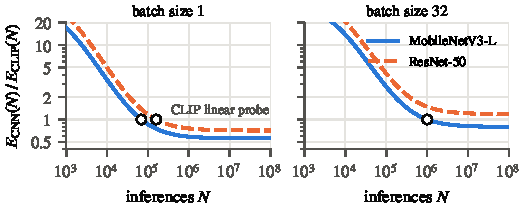
\includegraphics[width=\columnwidth]{figures/ratio_gross_fp16.pdf}
\caption{Life-cycle energy of the fine-tuned CNNs relative to CLIP with linear probe (gross, fp16).
Below 1 the CNN has used less energy in total; circles mark $N^{*}$.}
\label{fig:ratio}
\end{figure}

Accuracy and energy of all variants are given in Table~\ref{tab:variants}. The CNNs reach \SIrange{99.6}{99.7}{\percent} test accuracy and the linear probe \SI{98.7}{\percent}. Zero-shot CLIP is correct for
\SI{67.1}{\percent} of the test images, only 3.8 points above a constant \emph{defective}
answer. It detects 449 of the 453 defective parts, but 231 of the 262 good parts are rejected
as well. With the remaining two prompt sets, the accuracy falls to \SI{63.4}{\percent} and
\SI{43.5}{\percent}.

Fine-tuning takes about \SI{90}{s} for MobileNetV3 and \SI{104}{s} for ResNet-50. Between repetitions, the energy per
image differs by \SI{0.2}{\percent} at most. At batch size 1, kernel launches limit every model to 180
to 275 images per second, and the CPU package draws about \SI{33}{W}. At batch size 32, which
keeps the GPU busy, CLIP ViT-B/32 needs less energy per image than ResNet-50 (98.5 against
\SI{116.5}{mJ}), although torchvision lists about 4 GFLOPs per image for both (4.41 and
4.09).

The break-even points are shown in Table~\ref{tab:breakeven} and Fig.~\ref{fig:ratio}. In gross terms and at batch
size 1, the break-even against the linear probe lies at \num{6.9e4} inferences for MobileNetV3 and
at \num{1.6e5} for ResNet-50. A line inspecting one part per second reaches them after 19 and 44
hours. At batch size 32, MobileNetV3 saves only \SI{20}{mJ} per image, which moves
$N^{*}$ to \num{1.0e6} (about 12 days). Because ResNet-50 consumes \SI{18}{\percent} more
energy per image than CLIP, it never reaches a break-even. Against zero-shot CLIP, the values are at
most \SI{5}{\percent} higher, since the probe adds little training energy and costs the same per
inference. In net terms, the break-even points are 17 to \SI{28}{\percent} lower, and the conclusions
remain unchanged. If the energy is divided by accuracy, the break-even against the probe drops by less
than \SI{5}{\percent}, the one against zero-shot CLIP to half (\num{3.4e4} for MobileNetV3 at batch size 1).

\emph{Sensitivity.} In fp32, the per-image energy changes by a factor of 0.9 to 1.3 for MobileNetV3,
1.8 to 3.0 for ResNet-50 and 1.8 to 10.6 for CLIP, the larger value at batch size 32. All
break-even points against the probe then become finite and lie between \num{2.2e4} and \num{8.6e4}. Each seed reached its best validation F1 by epoch 5 of 10. Stopping there would have lowered $N^{*}$
at batch size 1 to about \num{1.9e4} and \num{2.9e4}.

\section{Discussion and Limitations}
On this dataset, zero-shot CLIP cannot serve as an inspection model, since it rejects
\SI{88}{\percent} of all good parts. The weak zero-shot performance agrees
with earlier findings for CLIP on specialised tasks~\cite{radford2021clip} and for plain CLIP prompts in
anomaly detection~\cite{zhou2024anomalyclip}. With \SI{0.6}{kJ} of training, the linear probe makes
up most of the accuracy deficit, but it requires labelled images. Zero-shot classification thereby loses
its main benefit, and the choice is between two supervised models, which makes the break-even against the probe the one
that matters in practice. The probe still makes about four times as many errors as
MobileNetV3 (1.3 against \SI{0.3}{\percent} of the test images). Dividing energy by accuracy weights false
rejects and escaped defects equally, although their costs differ and are not modelled.

Energetically, training pays off quickly on this machine. MobileNetV3
spends as much energy on training as on about \num{5.6e4} of its own single-image inferences.
Beyond roughly $10^{5}$ inspected parts, inference dominates and the cost per image decides. Recurring
retraining shifts this point but not the conclusion: with $k$ training runs over the service life,
$N^{*}$ grows by the factor $k$. The cost per image
is not proportional to the number of operations. ResNet-50 needs 19 times more FLOPs than MobileNetV3
but only 1.3 to 1.5 times more energy per image.
At batch size 1, kernel launches and the CPU are the bottleneck, consistent with the
finding that inference energy rises more slowly than FLOPs~\cite{desislavov2023trends}. The software
stack matters even more. Switching between fp16 and fp32 alone multiplied the per-image energy of CLIP
by up to 10.6 and turned an infinite break-even of ResNet-50 into \num{4.4e4} images. Energy figures of
models are therefore comparable only if precision, batch size and runtime are stated.

The main statements use gross values, since idle subtraction can magnify sensor
errors~\cite{fahad2019comparative}.

\emph{Limitations.} Only a single dataset was studied, on one machine and with one software stack
(PyTorch eager mode on ROCm). Optimised runtimes, CUDA graphs or quantisation were not used and would alter the energy per image,
above all at batch size 1. For supervised models, the dataset poses little difficulty, and it
is built from augmented variants of about 1,300 original images. In median cosine similarity of
CLIP features to the closest training image, test images (0.9925) and held-out validation images
(0.9930) are equally close. Leakage of augmented variants into the test set
can therefore not be ruled out. It would raise the accuracy of the CNNs and the probe, but not that of
zero-shot CLIP. Energy is read only from internal sensors: RAPL on AMD relies on a model~\cite{schoene2021zen2}, the
GPU sensor has not been checked externally, and RAM, mainboard and power supply are not
covered~\cite{jay2023softwaremeters}.
Since labelling effort and CLIP pre-training are not counted, the probe and zero-shot CLIP are
favoured. Only plain prompts were tested, while stronger methods such as
WinCLIP~\cite{jeong2023winclip} need more computation per image. The probe used all 5,969 training images, and few-shot probes were not examined.

\section{Conclusion}
For binary casting inspection, zero-shot CLIP is too inaccurate (\SI{67.1}{\percent}), so the realistic
alternative to a fine-tuned CNN is CLIP with a linear probe. MobileNetV3 is more accurate than this
probe (\SI{99.7}{\percent} against \SI{98.7}{\percent}) and recovers its \SI{21}{kJ} of training
after \num{6.9e4} single-image or \num{1.0e6} batched inferences. ResNet-50 pays off only at batch
size 1, because CLIP ViT-B/32 needs less energy per image in batched fp16 runs on this hardware. Batch
size, numerical precision and kernel support thus influence the break-even more than training energy
does, so it should be measured on the target hardware. A follow-up study should add a wall-plug meter,
optimised runtimes, edge hardware, more datasets and few-shot probes.

\bibliographystyle{IEEEtran}
\bibliography{refs}
\end{document}
